
%\hypertarget{aula-5}{%
%\chapter{Aula: 5}\label{aula-5}}




\hypertarget{retomando-aos-processos}{%
\chapter{Retomando aos processos}\label{retomando-aos-processos}}

Nas últimas, foram debatidos diversos aspectos dos processos dos SO
(Sistemas Operacionais). Esses aspectos orbitam os 3 pontos enfatizado a
seguir:

\begin{enumerate}
\def\labelenumi{\arabic{enumi}.}

\item
  Identificar os componentes de um processo.
\item
  Criação e Término de processos
\item
  Comunicação entre processos: \emph{Shared Memory} x \emph{Message
  Passing}.
\end{enumerate}

\hypertarget{componentes-de-um-processo.}{%
\subsection{Componentes de um
processo.}\label{componentes-de-um-processo.}}

Enquanto que um programa é uma entidade passiva localizada na memória
secundária, um processo é instância ativa de um programa, e está
localizado na memória principal em quatro sessões básicas (Como mostrado
na Figura \ref{fig:Processo na memória principal }): \emph{Text}, código executável; \emph{Data}, variáveis globais; \emph{Heap}, memória dinamicamente alocada; \emph{Stack},
armazenamento de dados temporários.



\begin{figure}[h!]
\centering
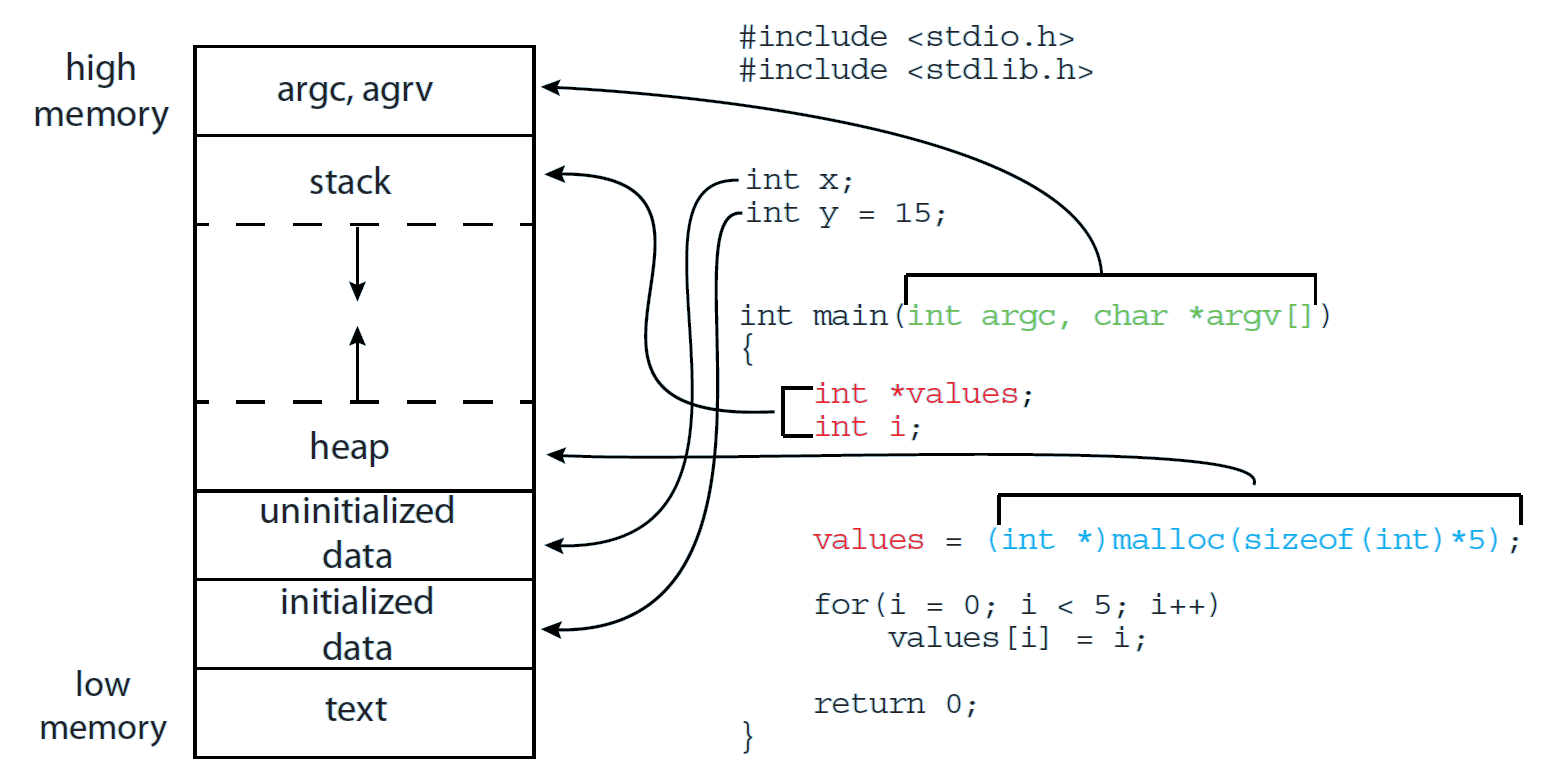
\includegraphics[keepaspectratio, width=12cm, height=9cm]{imagens/03/03 - Alocação de memória de um programa c.png}
\caption{Processo na memória principal \\
Imagem retirada de: Silberschatz, A. Operating System Concepts, 10th,
página 106. \\}
\label{fig:Processo na memória principal}
\end{figure}

Do ponto de vista do Sistema Operacional, cada processo é representado
pelo \emph{Process Control Block} (PCB), mostrado na Figura \ref{fig:PCB: Representação do processo no SO}, o qual
contém vários pedaços de informação necessários para iniciar ou
reiniciar um processo específico, como \emph{Process State},
\emph{Program counter}, \emph{CPU registers} e \emph{CPU-scheduling
information}.

\begin{figure}[h!]
\centering
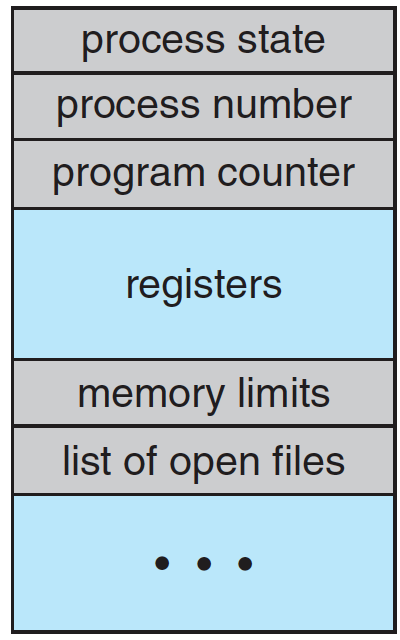
\includegraphics[keepaspectratio, width=12cm, height=9cm]{imagens/05/05 - Process Block Control (PCB).png}
\caption{PCB: Representação do processo no SO   \\
Imagem retirada de: Silberschatz, A. Operating System Concepts, 10th,
página 109 \\}
\label{fig:PCB: Representação do processo no SO}
\end{figure}



De forma geral, os processos podem assumir 5 estados (Como mostrado na
Figura \ref{fig:Estados de um process}): criado, pronto, rodando, esperando e terminado.


\begin{figure}[h!]
\centering
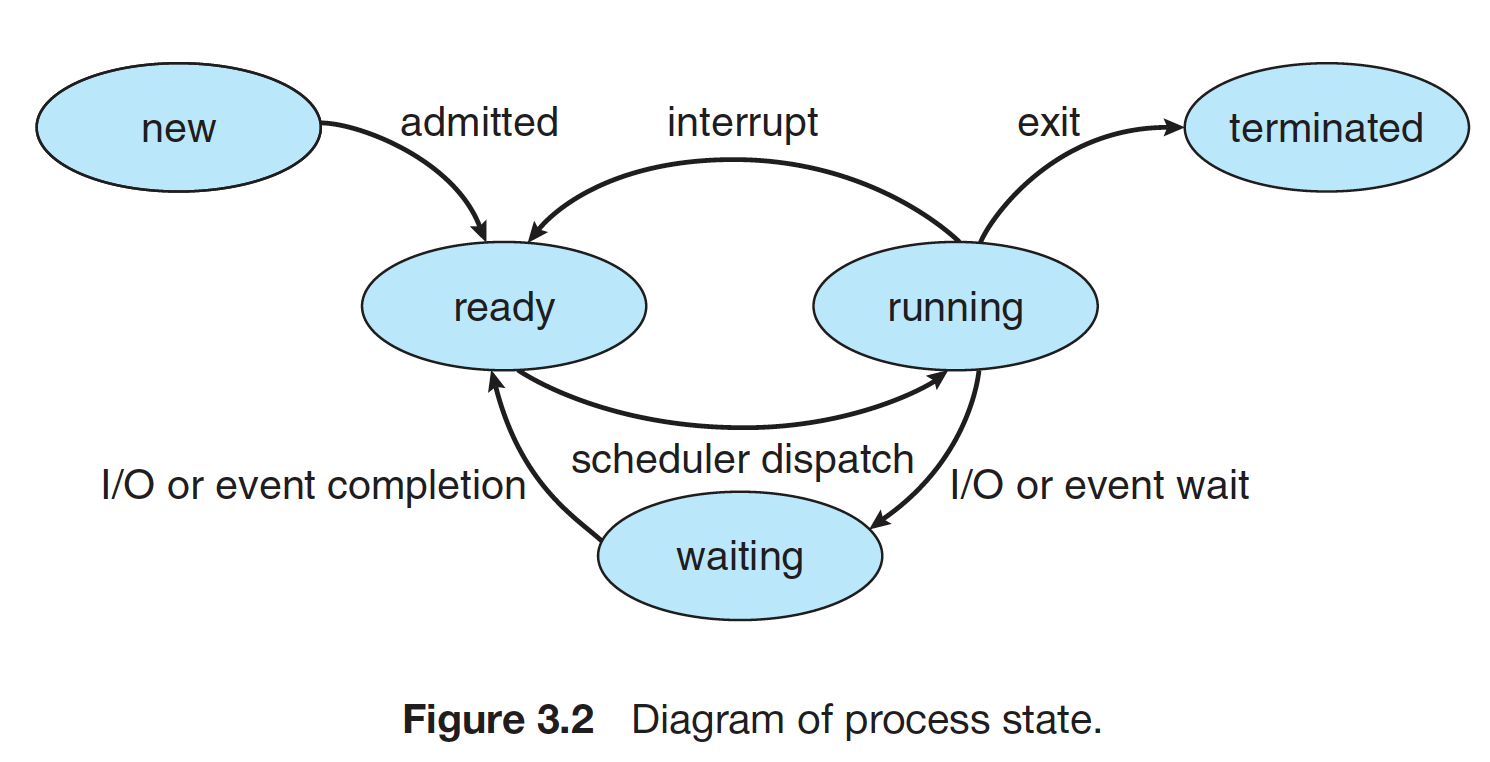
\includegraphics[keepaspectratio, width=12cm, height=9cm]{imagens/05/05 - Diagram of Process State.png}
\caption{Estados de um processo   \\
Imagem retirada de: Silberschatz, A. Operating System Concepts, 10th,
página 109. \\}
\label{fig:Estados de um process}
\end{figure}


No Linux, todos os PCB's encontram-se em uma lista duplamente encadeada
(com o próximo e o anterior), com o sistema operacional armazenando um
ponteiro para a estrutura que está atualmente em execução pela CPU.
Mostrado na Figura \ref{fig:Representação da fila encadeada}.


\begin{figure}[H]
\centering
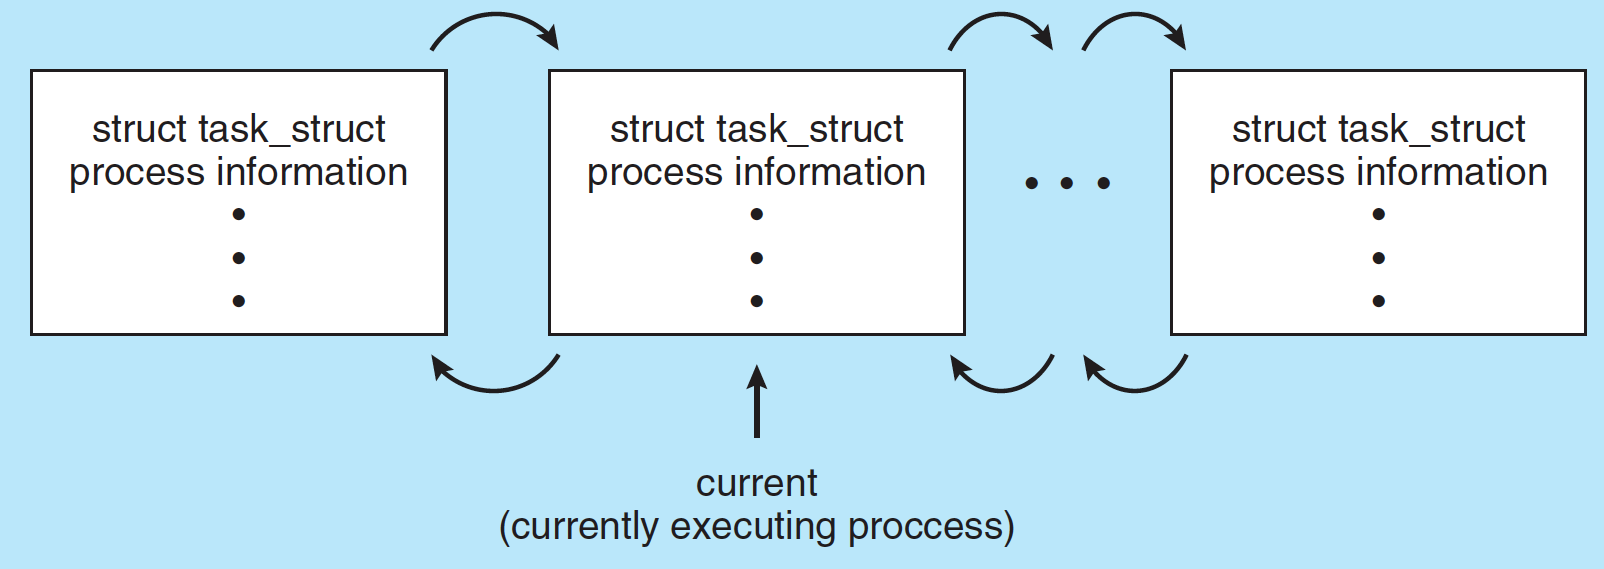
\includegraphics[keepaspectratio, width=12cm, height=9cm]{imagens/05/05 - Representacao da fila encadeada.png}
\caption{Representação da fila encadeada   \\
Imagem retirada de: Silberschatz, A. Operating System Concepts, 10th,
página 111. \\}
\label{fig:Representação da fila encadeada}
\end{figure}



Conforme o estado do processo muda, o PCB também muda de fila,
alternando entre a fila encadeada de ``pronto'' (pronto para ser
executado) e espera (espera de ocorrência de evento), mostradas na
Figura \ref{fig:Filas de espera e pronto}.

\begin{figure}[h!]
\centering
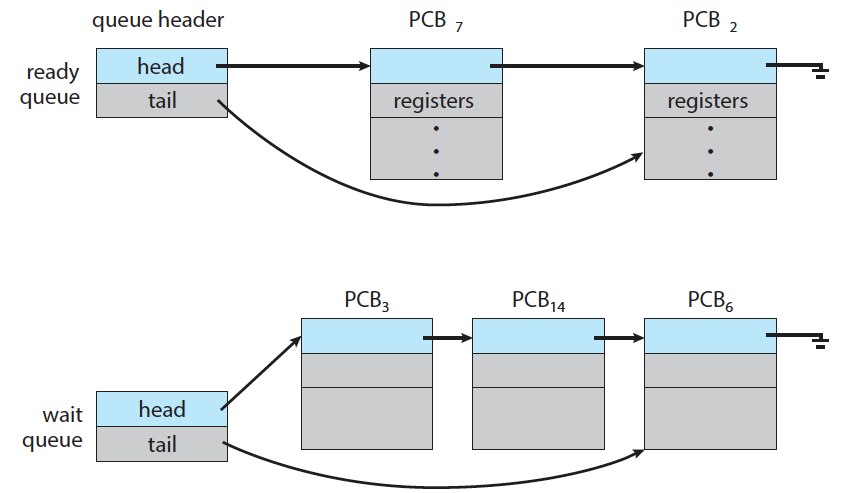
\includegraphics[keepaspectratio, width=12cm, height=9cm]{imagens/05/05 - Filas de espera e pronto.png}
\caption{Filas de espera e pronto   \\
Imagem retirada de: Silberschatz, A. Operating System Concepts, 10th,
página 112. \\}
\label{fig:Filas de espera e pronto}
\end{figure}



O responsável por depositar e recolher os PCB's dessas filas é o
\emph{process Scheduling}, o qual foi representado no diagrama da Figura
\ref{fig:Diagrama de agendamento de processos}.


\begin{figure}[h!]
\centering
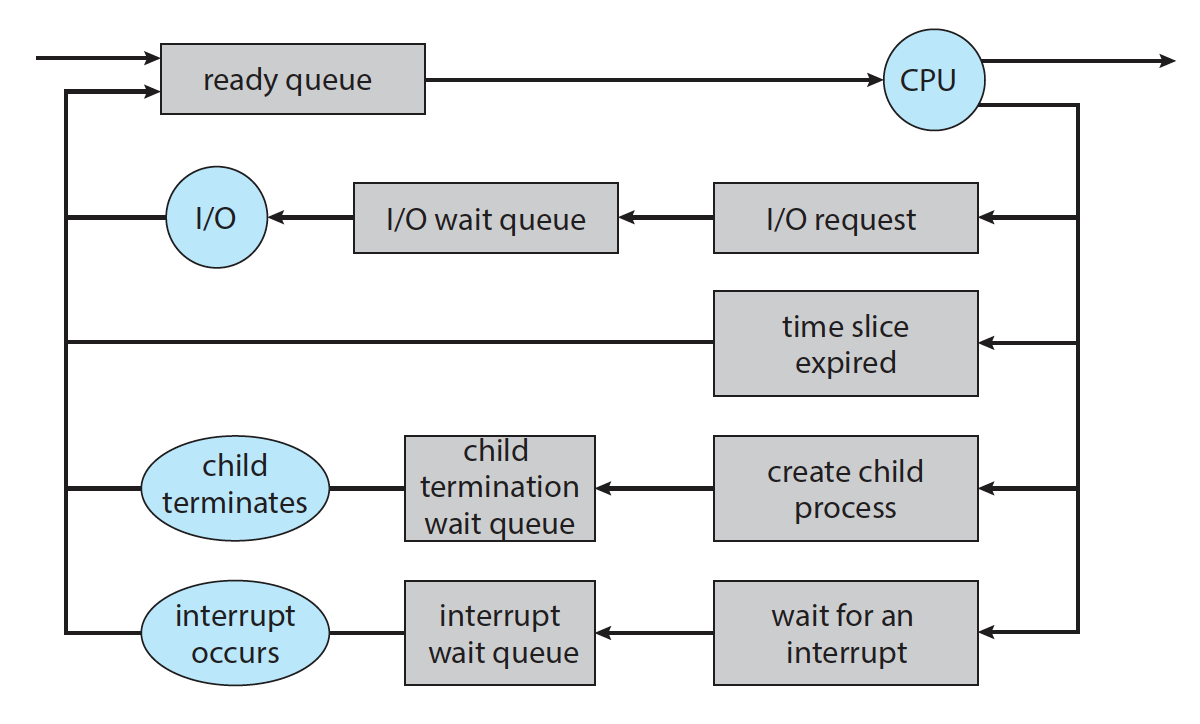
\includegraphics[width=12cm, height=9cm]{imagens/05/05 - Diagrama Agendamento de Processos.png}
\caption{Diagrama de agendamento de processos   \\
Imagem retirada de: Silberschatz, A. Operating System Concepts, 10th,
página 113. \\}
\label{fig:Diagrama de agendamento de processos}
\end{figure}


O \emph{CPU Scheduling}, por sua vez, tem como papel recolher um
processo da fila \emph{ready} para um núcleo de processamento. Para ser
alocado na CPU, é necessário salvar o estado do processo anteriormente
alocado, bem como os elementos necessários para continuar processando-o
posteriormente, e carregar o novo contexto de execução. No decorrer
dessa tarefa, chamada de \emph{Context Switch}, a CPU fica ociosa, como
mostra a Figura \ref{fig:Diagrama da troca de contexto}.

\begin{figure}[h]
\centering
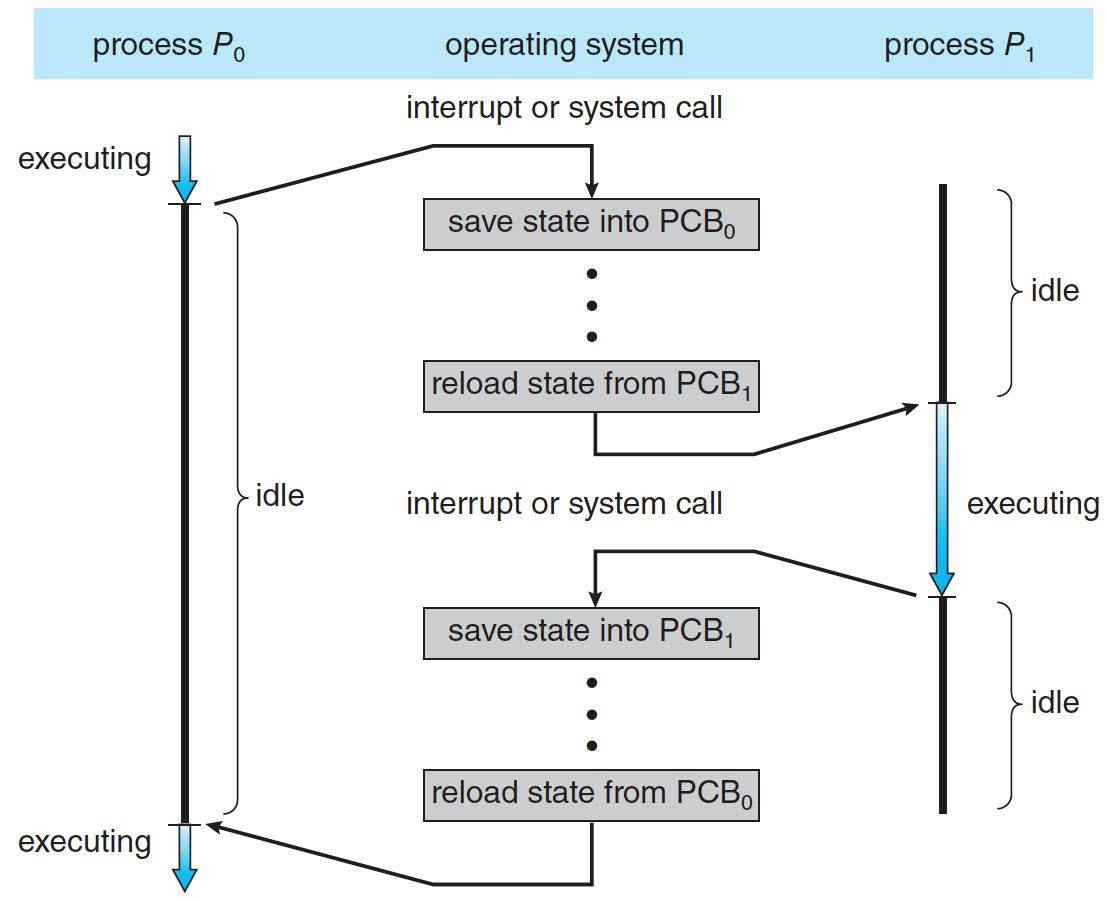
\includegraphics[keepaspectratio, width=12cm, height=9cm]{imagens/05/05 - Diagrama Contex Switch.png}
\caption{Diagrama da troca de contexto   \\
Imagem retirada de: Silberschatz, A. Operating System Concepts, 10th,
página 113. \\}
\label{fig:Diagrama da troca de contexto}
\end{figure}


\hypertarget{criauxe7uxe3o-e-tuxe9rmino-de-um-processo.}{%
\subsection{Criação e Término de um
processo.}\label{criauxe7uxe3o-e-tuxe9rmino-de-um-processo.}}

Cada processo tem uma identificação única chamada de \texttt{pid}
(\emph{process identifier}). A partir dele pode ser criado um processo
filho. Conscutivas criações formam uma árvore de processos, mostrada na
Figura \ref{fig:Árvore de processos típico de sistema Linux}.


\begin{figure}[H]
\centering
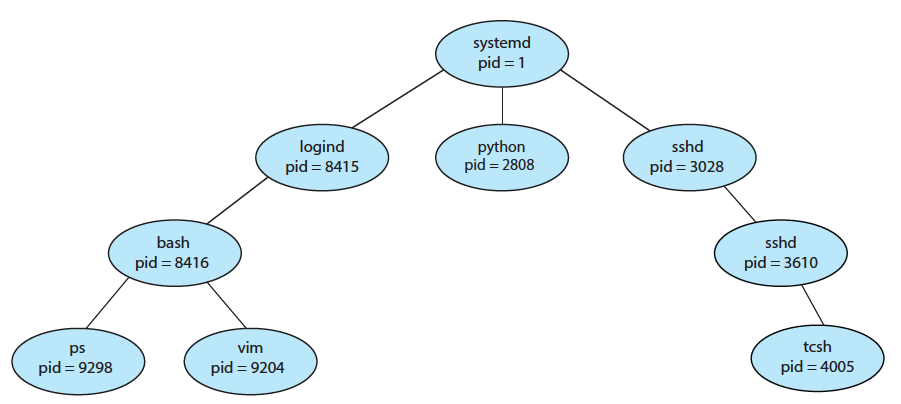
\includegraphics[width=8cm, height=5cm]{imagens/05/05 - Arvore de processos em um sistema linux.png}
\caption{Árvore de processos típico de sistema Linux   \\
Imagem retirada de: Silberschatz, A. Operating System Concepts, 10th,
página 116. \\}
\label{fig:Árvore de processos típico de sistema Linux}
\end{figure}


O ciclo de criação e término de um processo, mostrado na Figura \ref{fig:Criação e término de um processo}, passa
pelas funções de chamada de sistema na linguagem \texttt{C}:
\texttt{fork()}, para criar um novo processo; \texttt{wait()}, esperar o
processo filho acabar; \texttt{execve()}, troca a imagem de execução
(troca o programa); \texttt{exit()}, encerrar o processo.


\begin{figure}[h!]
\centering
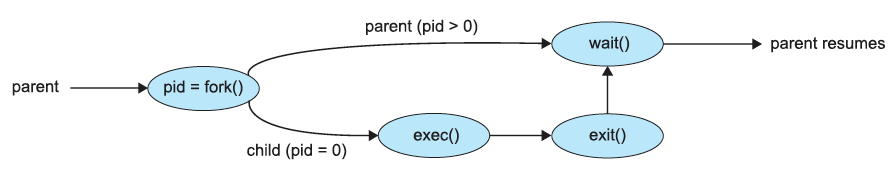
\includegraphics[keepaspectratio, width=15cm, height=17cm]{imagens/05/05 - Process Creation.png}
\caption{Criação e término de um processo   \\
Imagem retirada de: Silberschatz, A. Operating System Concepts, 10th,
página 119. \\}
\label{fig:Criação e término de um processo}
\end{figure}


Alguns sistemas não permitem que um processo ``viva'' sem que o ``pai''
exista. Então, se o ``pai'' for encerrado, todos os ``filhos'' serão
encerrados. Da mesma forma que os filhos dos filhos. Fenômeno chamado de
\emph{cascading termination}

Ao chamar a função \texttt{exit()}, um processo filho tem seus recursos
deslocados pelo sistema operacional. Porém ele continua na tabela de
processos até o processo pai executar a função \texttt{wait()}, pois
nessa tabela está contido o estado de saída do mesmo. Durante essa
transição, de seus recursos terem sido deslocados mas ainda estar na
tabela de processos, o processo é chamado de \texttt{Zumbie}, o que,
normalmente, ocorre para todos os processos (ao serem terminados) por um
curto período de tempo. Se o pai não chamar a função \texttt{wait()} e
terminar sua execução, os processos filhos passarão a ser chamados de
processos \texttt{órfãos}. O Sistema Operacional Linux utiliza de outros
processos para herdar os \texttt{órfãos} e libera-los da tabela de
processos chamando a função \texttt{wait()}.

\hypertarget{comunicauxe7uxe3o-entre-processos-shared-memory-x-message-passing.}{%
\section{\texorpdfstring{Comunicação entre processos: \emph{Shared
Memory} x \emph{Message
Passing}.}{Comunicação entre processos: Shared Memory x Message Passing.}}\label{comunicauxe7uxe3o-entre-processos-shared-memory-x-message-passing.}}

Um processo pode ter sido criado com o objetivo de executar um algoritmo
que independe de outros processos (esse processo é chamado de
independente). Ou, pode ter sido criado para cooperar com outros
processos (esse processo é chamado de cooperativo). Para que a
cooperação ocorra, é necessário criar um canal de comunicação (um
\emph{Interprocess Communication - IPC} ), de tal maneira que os dados
possam ser transmitidos de uma para outra. Há dois métodos para tal: o
\emph{Shared Memory} (compartilhamento de memória); e o \emph{Message
Passing} (sistema de passagem de mensagem).

Há várias razões para ter um processo cooperativo. 1. Troca de
informações: Compartilhamento de informações entre os interessados. 2.
Aceleração computacional: Dividir uma tarefa em várias pequenas partes
e, assim, processá-los ao mesmo tempo. 3. Modularidade: Com as funções
do sistema dividido em diferentes processos ou threads.

\hypertarget{shared-memory}{%
\subsection{Shared Memory}\label{shared-memory}}

\emph{Shared Memory} é o método que torna uma faixa de endereços de
memória acessível à diferentes processos. Por questões de segurança, o
sistema operacional (de forma padrão) não permite que os processos
tenham acesso aos espaços de memória dos outros. Para que esse método
ocorra, é fundamental que todos os processos participantes desse método
concordem em compartilhar a sua faixa de memória. Após executado, o
sistema operacional não mais intervem, deixando para os processos a
responsabilidade de garantir que não ocorra o problema chamado
\emph{Race Conditions} (ou condição de disputa).

O \emph{Race Conditions} decorre de um problema de \emph{concurrency}
(simultaneidade) entre os diferentes processos, como a escrita em um
mesmo endereço de memória transcorrendo por mais de um processo ao mesmo
tempo.

Uma solução para garantir a comunicação entre os processos é utilizando
a arquitetura \emph{producer-consumer}, no qual o processo
\emph{producer} produz e armazena o conteúdo em um buffer, que será
consumido pelo \emph{consumer} posteriormente. Esse \emph{buffer} pode
ser \emph{unbounded buffer} (não tem limites de tamanho) ou
\emph{bounded buffer} (com o tamanho limitado).

\hypertarget{message-passing}{%
\subsection{Message Passing}\label{message-passing}}

A idéia por de trás do método \emph{message passing} é a de passar a
responsabilidade da distribuição e validade da comunicação
inter-processual para o sistema operacional, promovendo uma abstração de
uso facilitado (em comparação ao \emph{shared memory}), pois descarta a
necessidade da criação explícita de um código de gerenciamento de acesso
e manupulação dos dados compartilhados. Esse mecanismo de comunicação
cria um elo de ligação (\emph{link}) entre dois processos, que demanda
ao menos duas operações: \emph{send(message)}; e
\emph{receive(message)}.

A implementação desse método passa por 3 pontos:

\begin{enumerate}
\def\labelenumi{\arabic{enumi}.}
\tightlist
\item
  Comunicação direta e indireta.
\item
  Síncrona ou assíncrona.
\item
  \emph{Buffer} automático ou explícito.
\end{enumerate}

\hypertarget{comunicauxe7uxe3o-direta}{%
\subsubsection{Comunicação Direta}\label{comunicauxe7uxe3o-direta}}

Na comunicação direta, o processo deve nomear explicitamente o nome do
receptor ou emissor: 1. \emph{send(P, message)}: Enviar menssagem para o
processo P 2. \emph{receive(Q, message)}: Receber mensagem do processo Q

\hypertarget{comunicauxe7uxe3o-indireta}{%
\subsubsection{Comunicação indireta}\label{comunicauxe7uxe3o-indireta}}

Na comunicação indireta, as mensagens passam através de uma abstração de
caixa de correios (\emph{mailbox} ou \emph{ports}) compartilhada, na
qual as mensagens podem ser postadas e removidas. Cada \emph{mailbox}
tem uma identificação única (no POSIX, cada \emph{mailbox} é
identificado por um inteiro). Nessa implementação, o processo deve
nomear de qual e para qual caixa de correios deve enviar ou receber a
mensagem:

\begin{enumerate}
\def\labelenumi{\arabic{enumi}.}
\tightlist
\item
  \emph{send(A, message)}: Enviar uma mensagem para o \emph{mailbox} A.
\item
  \emph{receive(A, message)}: Receber uma mensagem do \emph{mailbox} A.
\end{enumerate}

Um possível \emph{Race Condition} ocorre quando o processo P1 envia uma
mensagem, e o P2 e P3 estão chamando a função \texttt{receive()}. Para
evitar que isso aconteça, existem 3 possibilidades:

\begin{enumerate}
\def\labelenumi{\arabic{enumi}.}
\tightlist
\item
  Permitir que somente 2 processos estejam associados à uma caixa de
  correios.
\item
  Permitir que somente 1 processo por vez execute a função
  \texttt{receive()}
\item
  Permitir que o sistema operacional escolha qual processo deve receber
  (P1 ou P2, mas não ambos).
\end{enumerate}

\hypertarget{sincronia}{%
\subsubsection{Sincronia}\label{sincronia}}

Para cada um dos dois primitivos (\texttt{send()} e \texttt{receive()}),
o sistema de transmissão de mensagens pode assumir 2 estados, o síncrono
e o assíncrono:

\begin{enumerate}
\def\labelenumi{\arabic{enumi}.}
\item
  Síncrono (\emph{Blocking} ou bloqueante): 1.1. O emissor (P1) é
  travado até o receptor (P2) receber a mensagem. 1.2. O receptor (P1) é
  travado até uma mensagem ficar disponível.
\item
  Assíncrono (\emph{Nonblocking} ou não-bloqueante) 2.1. O emissor (P1)
  continua a executar suas instruções após a emissão da mensagem. 2.2. O
  receptor (P2) pode receber uma mensagem inválida (NULL), assim
  continuar sua execução mesmo sem ter recebido uma mensagem válida.
\end{enumerate}

\hypertarget{buffer}{%
\subsection{Buffer}\label{buffer}}

Todas as mensagens enviadas devem passar por um sistema de fila que,
basicamente, tem 3 formas distintas (que apenas variam sua capacidade):

\begin{enumerate}
\def\labelenumi{\arabic{enumi}.}
\tightlist
\item
  Capacidade 0 (\emph{Zero capacity} ou sem \emph{buffer}): O emissor
  deve ser síncrono com o receptor, caso contrário a mensagem será
  perdida.
\item
  Capacidade limitada (\emph{Bounded capacity}): O emissor pode ser
  assíncrono caso haja capacidade de armazenamento de mensagens no
  \emph{buffer}. E, caso a fila esteja cheia, deve ser bloqueado até
  haver espaço disponível.
\item
  Capacidade ilimitada (\emph{Unbounded capacity}): O emissor nunca é
  bloqueado, pois a fila não tem limites de recepção de mensagens.
\end{enumerate}

\hypertarget{complementar-1}{%
\section{Complementar}\label{complementar-1}}

Essa sessão faz alusão à outros conteúdos também importantes
relacionados com a aula, mas que dará ao leitor o papel de buscar mais
informações sobre os mesmos conforme sua necessidade e interesse.

\hypertarget{threads---criauxe7uxe3o-em-c}{%
\subsection{\texorpdfstring{Threads - criação em
\texttt{C}}{Threads - criação em C}}\label{threads---criauxe7uxe3o-em-c}}

Nas aulas anteriores foram discutidos as vantagens das threads em
comparação aos processos. Abaixo está um código comentado em \texttt{C}
para criação de threads.

\begin{minted}[mathescape, linenos]{c}

    #include <stdio.h>
    #include <pthread.h> //POSIX thread library, or pthread.
    
    
    int sum;
    void *runner(void *param);
    
    int main(int argc, char *argv[])
    {
            pthread_t tid;
            pthread_attr_t attr;
            
            pthread_attr_init(&attr); 
            //Atributo necessário para a criação da thread
            
            /*
             * pthread_create
             * tid vai retornar o 'id' da thread. 
             * runner é a função que será executada
             * argv[1] é o argumento no qual será passado para a função runner
             *
             */
            pthread_create(&tid, &attr, runner, argv[1]); 
            pthread_join(tid, NULL); //Espera uma thread Terminar
            
            return 0;
    }
    
    void *runner(void *param){
            
            int upper = atoi(param);
            int sum = 0;
            
            for(int i = 0; i < upper; i++){
                   sum += 1;
            }
            
            pthread_exit(0);
    }
\end{minted}



\hypertarget{pesquisar-sobre-1}{%
\subsection{Pesquisar Sobre}\label{pesquisar-sobre-1}}

\begin{enumerate}
\def\labelenumi{\arabic{enumi}.}

\item
  Teoria de filas
\item
  \emph{pipes} (mecanismo \emph{IPC - InterProcess Communication}) -
  Página 139 (Capítulo 3.7) de Silberschatz, A. Operating System
  Concepts, 10th.
\end{enumerate}
